\section{Cytologie}

\subsection{Basics}

	\begin{itemize}
		\item Domänen: Bacteria, Archaea und Eukarya
		\item Verhältnis Oberfläche/Volumen 
	\end{itemize}

	In Tabelle \ref{tab:domaenenuberblick} ist eine Übersich über die Eigenschaften der drei Organismenreiche.	

	\begin{table}[h!]
	\begin{center}
	\begin{tabular}{l l l l} 
	\toprule
	Merkmal		&	Bacteria		&	 Archaea				&	 Eukaraya		\\
	\midrule
	Zellkern 	&	nein			&	 nein					&	 ja		\\
	cccDNA		&	ja				&	 ja					&	 nein (linear)			\\
	Histone		&	nein			&	 ja					&	 ja		\\
	Zellwand		&	Murein		&	 kein Murein		&	 kein Murein		\\
	Membranlipid&	Ester			&	 Ether				&	 Ester		\\
	\midrule
	Ribosomen	&	70S			&	 70S					&	 80S		\\
	Ini-tRNA		&	f-Met			&	 Met					&	 Met		\\
	Introns 		&	nein			&	 nein					&	 ja		\\
	ja				&	Operon		&	 ns					&	 nein		\\
	Cap/poly-A 	&	nein			&	 nein					&	 ja		\\
	Plasmide		&	ja				&	 ja					&	 selten		\\
	RNA-Pol			&	ne (4 UE)	&	 viele (8-12 UE)	&	drei (12-14 UE)	\\
	TK-Faktoren		&	nicht nötig	&	 benötigt			&	benötigt		\\
	Promotoren		&	-10, -35		&	 TATA					&	TATA		\\
	\midrule
	Methanbildung		&	nein			&	 ja					&	nein		\\
	S-Reduktion		&	ja				&	 ja					&	nein		\\
	Nitrifizierung	&	ja				&	 nein					&	nein		\\
	Denitrifizierung		&	ja				&	 ja					&	nein		\\
	N-Fixierung		&	ja				&	 ja					&	nein		\\
	Photosynthese		&	ja				&	 nein					&	nein (Plastiden)	\\
	Lithotrophie	&	ja				&	 ja					&	nein		\\
	Grw. > 80°C		&	ja				&	 ja					&	nein		\\
	\bottomrule
	\end{tabular}
	\caption{Übersicht über die Eigenschaften der drei Organismenreiche.}
	\label{tab:domaenenuberblick}
	\end{center}
	\end{table}

\subsection{Aufbau}

	\begin{figure}[ht!]
	\leavevmode
	\begin{center}
	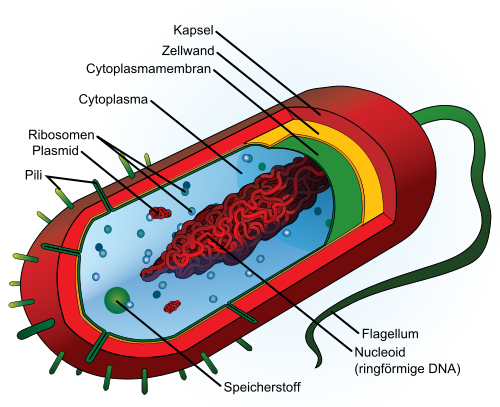
\includegraphics[scale=0.47]{./pictures/avg_prokaryote_cell_500}
	\end{center}
	\caption{\slshape{Typische prokaryotische Zelle.}}
	\label{fig:prokarya}
	\end{figure}

	\begin{figure}[ht!]
	\leavevmode
	\begin{center}
	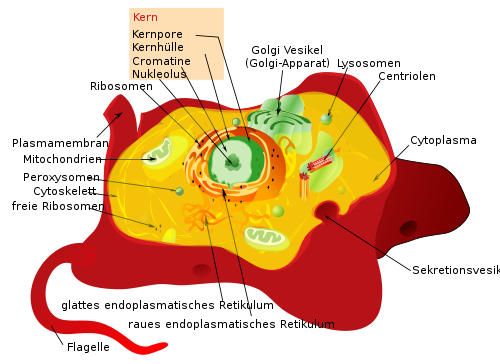
\includegraphics[scale=0.47]{./pictures/animal_cell_500}
	\end{center}
	\caption{\slshape{Tierische Zelle als Beispiel einer eukaryotischen Zelle.}}
	\label{fig:eukarya}
	\end{figure}


\subsection{Membran}
\begin{description}
	\item[Einheitsmembranen (unit membrane)] \hfill \\
		\begin{itemize}
			\item Doppelschicht aus amphiphilen Fettsäuren (5 nm)
			\item ungesättigte Fettsäuren führen zu erhöhter Fluidität
			\item Temperaturanpassung: Cholesterin (Eukarya), Hopanoide (Prokarya)
			\item Funktion: Permeabilitätsbarriere, Proteinverankerung, Energiekonservierung
		\end{itemize}

	\item[Äußere Membran (outermembrane)] \hfill \\
		\begin{itemize}
			\item Peptidoglycanschicht
			\item Periplasma
		\end{itemize}
	
\end{description}

\subsection{Zellwand}
